\begin{figure}[htbp]
\centering
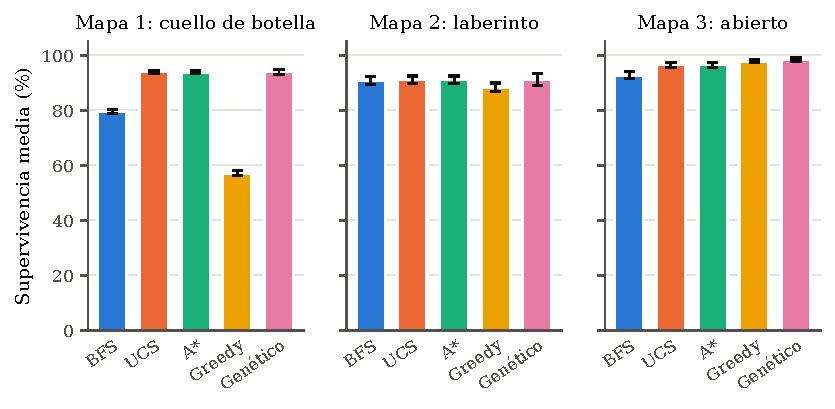
\includegraphics[width=\textwidth]{figuras/supervivencia.pdf}
\caption{Tasa de supervivencia media por mapa y algoritmo. Las barras de error indican el intervalo de confianza del 95\,\% de la media.}
\label{fig:supervivencia}
\end{figure}

\begin{figure}[htbp]
\centering
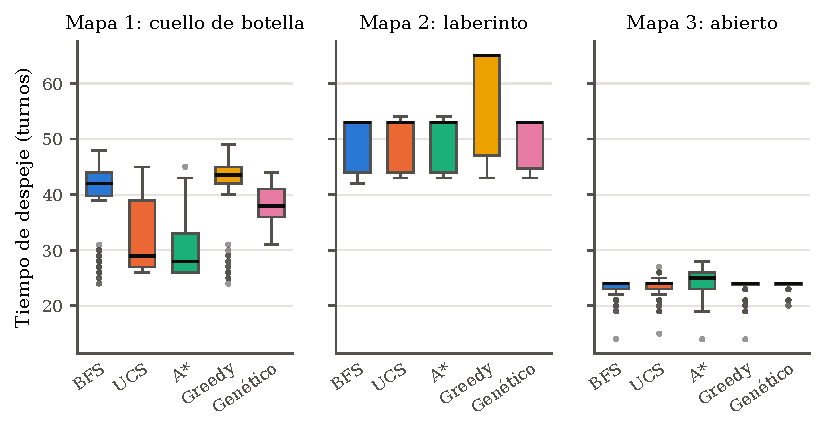
\includegraphics[width=\textwidth]{figuras/tiempo_despeje.pdf}
\caption{Distribución del tiempo de despeje (turnos hasta que evacúa el último sobreviviente) por mapa y algoritmo.}
\label{fig:tiempo_despeje}
\end{figure}

\begin{figure}[htbp]
\centering
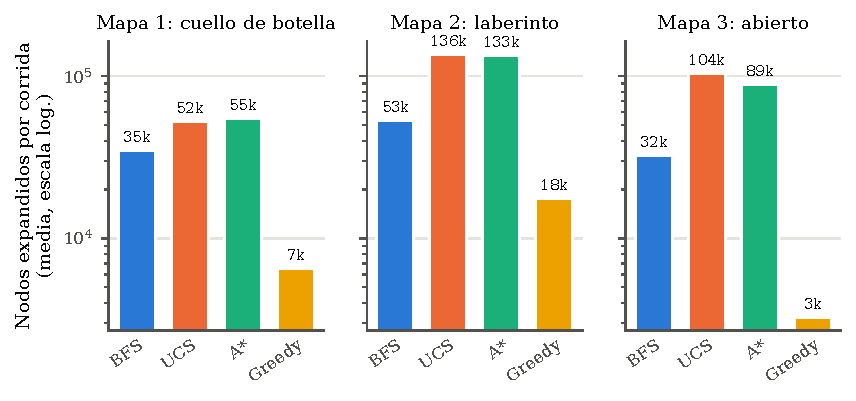
\includegraphics[width=\textwidth]{figuras/nodos_expandidos.pdf}
\caption{Nodos expandidos por corrida de simulación (media, escala logarítmica), sumando todas las replanificaciones. No incluye el algoritmo genético, cuyo costo está en las simulaciones de evaluación de aptitud.}
\label{fig:nodos_expandidos}
\end{figure}

\begin{figure}[htbp]
\centering
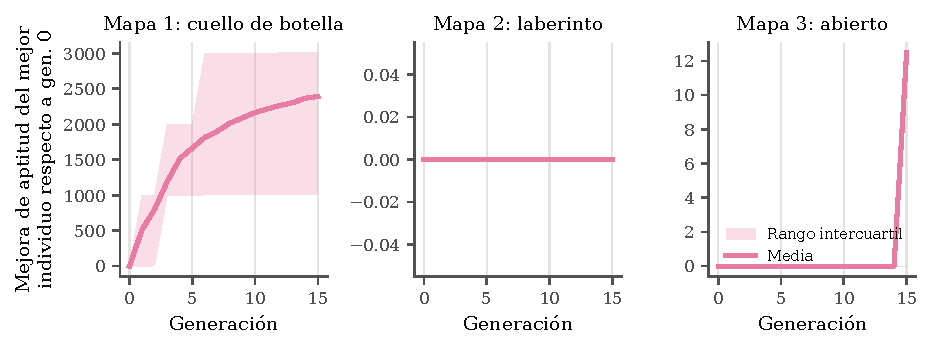
\includegraphics[width=\textwidth]{figuras/convergencia_genetico.pdf}
\caption{Convergencia del algoritmo genético: mejora de la aptitud del mejor individuo respecto a la generación inicial.}
\label{fig:convergencia_genetico}
\end{figure}
